% ------------------------------------------------------ %
%                 请使用XeLaTeX进行编译!!!
% ------------------------------------------------------ %
%         本项目我已开源在Github上:
%         https://github.com/XingA02/cls_for_CUMCM
%         个人Github主页:https://github.com/XingA02
% ------------------------------------------------------ %
\documentclass{xtan_cumcm}


\begin{document}   % 文章开始



% ----------------------------------------------- %
%              请在这里输入文章标题
% ----------------------------------------------- %
%              请在这里输入文章标题
% ----------------------------------------------- %
\title{数学建模内容参考模板}\author{}\date{}\maketitle\vspace{-5em}  




% ---------------------------------------------------- %
%  打开chapter文件夹里的“0-摘要.tex”文件,编辑其中的内容
% ---------------------------------------------------- %
\begin{abstract}

    摘要是全文最重要的部分,也是阅卷人首先看到的部分,阅卷人会只根据摘要将文章分成三六九等,所以如果不认真写摘要的话你就会有大麻烦,请务必留至少两小时用于摘要的打磨,将其控制在1面!!!
    
    针对问题一:在写摘要的时候请搞清楚,首先摘要的第一段是题设的背景,你需要随便胡扯几句,但别扯太多,毕竟要把摘要控制在一面很难!然后写完第一段后从第二段开始就要开始介绍你对每个题目的理解、过程以及求解与评价,语言尽量精炼,不要啰嗦,再强调一次:那么多内容的摘要压缩在一面非常难!下面我将给大家演示如何对于自己已经完成的“模型建立与求解”部分进行摘要描述。
    
    针对问题二,本文基于可视化和假设检验对所给数据集进行数据分析。首先对产品的销售价格和销售量的关系进行探究,本文分别通过\textbf{斯皮尔曼相关系数}对相关性进行定量描述,求得$\rho$=-0.2946,反映出\textbf{销售价格和销售量的相关性较弱}。接着对区域与销量的关系进行探究,通过\textbf{方差检验}得知\textbf{不同地区对订单的需求量有显著差异},并通过直方图探究出不同区域产品的需求量的不同特性。然后,本文对产品的销售方式与需求量的关系进行探究,通过\textbf{Mann-Whitney U}检验得出\textbf{线上销售与线下销售的销售量存在显著差异}。最后,通过\textbf{单样本Wilcoxon符号秩检验}将时间序列整体与促销活动单日的销量相比较,得出\textbf{促销活动单日的销量与平时的销量有显著差异}。为了将各特征的分布以及定量分析所得出的结论直观化,本文利用小提琴图、箱线图、直方图等对相关特征进行可视化,结果与定量分析一致。
    
    针对问题三,我认为摘要关于每个题的内容应该有以下特点:整段的写作应该是循序渐进的,比如使用“首先本文XXX”、“接着本文XXX”、“然后本文XXX”以及“最后本文XXX”这样的形式;\textbf{关键的方法和结论}应该是加粗显示,\LaTeX 在文中的加粗的代码想必大家已经看到了;段落中除了写建模过程中我们用了什么方式做了什么,还应该描述结论——定性的结论要直接给出,定量的结论如果较多可以概括性描述。
    
    针对问题四,最后说一说关于这个模板,我认为数学建模竞赛的结果与论文的关联性是非常强的,所以不应该一味追求技术的实现,应该尤其重视文章的撰写与排版,\LaTeX 作为一个非常经典的排版工具有一定的上手门槛,如果大家使用好了可以给文章加分不少,但是务必在比赛前多尝试,尤其是把自己之前的论文套入模板看看是否会出问题,否则比赛的时候如果花大量的时间摆弄\LaTeX ,那就是得不偿失了。
    
    \vspace{1em} % 移除2个行距的空白:这句代码千万不能动!!!移除2个行距的空白:这句代码千万不能动!!!
    
    \noindent{\textbf{关键词:}随机森林;方差选择法;Voting Classifier;层次聚类分析;决策树}
    
\end{abstract} 


% 本行代码会删除第一页(标题与摘要页)的页码,仅在需要目录的时候解除注释
% \thispagestyle{empty}


\newpage


% 数学建模国赛要求不能有目录,下面这行代码仅在需要目录的时候解除注释
%\tableofcontents\thispagestyle{empty}\newpage\setcounter{page}{1}


\pagestyle{fancy}\fancyhead{}\fancyfoot[C]{\thepage}





% ---------------------------------------------------------- %
% 接下来的部分即为文章每个章节的内容,记住一个准则:
% 有多少个章节就在chapter文件夹中制作多少个tex文件,
% 每个文件管一个章节就行啦!!!
% ---------------------------------------------------------- %



% ---------------------------------------------------------- %
%    打开chapter文件夹里的“1-问题重述.tex”文件,编辑其中的内容
% ---------------------------------------------------------- %
\section{问题重述}

\subsection{问题背景}

数学建模比赛论文是要我们解决一道给定的问题,所以正文部分一般应从问题重述开始,一般确定选题后,写手就可以开始写这一部分了——毕竟这个部分不需要等编程手和建模手掰扯。

这部分的内容是将原问题进行整理,将问题背景和题目分开陈述即可,所以基本没啥难度——问题背景就是把赛题给出的具体背景简要的阐释并加上具体的理解,问题提出就是把3(4)个小题用自己的话复述一遍。

本部分的目的是要吸引读者读下去,所以文字不可冗长,内容选择不要过于分散、琐碎,措辞要精练。
注意:在写这部分的内容时,绝对不可照抄原题!(论文会查重)
应为:在仔细理解了问题的基础上,用自己的语言重新将问题描述一遍。语言需要简明扼要,没有必要像原题一样面面俱到。


\subsection{问题提出}


下面我将给出2022年数学建模国赛C题的“问题提出”示例供大家参考。现有一组由专家给出的关于玻璃的数据,要求通过分析与建模解决下面若干问题:

\textbf{问题1:} 分析这些玻璃文物的表面风化与其玻璃类型、纹饰和颜色的关系以及文物样品表面有无风化化学成分含量的统计规律,并对风化前的化学含量进行分析。

\textbf{问题2:} 依据附件数据分析两种玻璃的分类规律;对于每个类别选择合适的化学成分进行亚类划分,给出划分方法及结果,并分析分类结果的合理性和敏感性。 

\textbf{问题3:} 分析未知类别玻璃文物的化学成分,鉴别其所属类型并对分类结果的敏感性进行分析。 

\textbf{问题4:} 针对不同类别的玻璃文物样品,分析其化学成分之间的关联关系并对其差异性进行比较。


% ---------------------------------------------------------- %
%    打开chapter文件夹里的“2-问题分析.tex”文件,编辑其中的内容
% ---------------------------------------------------------- %
\section{问题分析}

\subsection{问题一的分析}

从实际问题到模型建立是一种从具体到抽象的思维过程,问题分析这一部分就是沟通这一过程的桥梁,因为它反映了建模者对于问题的认识程度如何,也体现了解决问题的雏形,起着承上启下的作用,也很能反应出建模者的综合水平。

这部分的内容应包括:题目中包含的信息和条件,利用信息和条件对题目做整体分析,确定用什么方法(并不是具体的算法和模型)建立模型,假如我后面要对数据进行清洗、特征缩放、特征编码然后建模,我不能在这里说我要怎么处理缺失值、异常值,也不能说我要用独热编码、要用数据归一化,更不能说我要用SVM、要用树模型啦,而是应该说“本文首先对数据集进行合理的数据预处理与特征工程,并建立分类模型实现预测……”。一般是每个问题单独分析一小节,分析过程要简明扼要, 不需要放结论。

建议在文字说明的同时用图形或图表(例如流程图)列出思维过程,这会使你的思维显得很清晰,让人觉得一目了然!接下来我给出2023年数学建模国赛C题的“问题分析”示例供大家参考。




\subsection{问题二的分析}

\textbf{针对问题二},第一小问要求分析各蔬菜品类的销售总量与成本加成定价的关系。首先为了便捷分析,将四个附件的数据信息合并;接着按日聚合数据并将销售量并求和,并取销售单价的均值;然后采用孤立森林模型清洗异常值。因数据未提供成本加成定价,所以首先计算出此数值。接着采用多项式回归拟合模型,输出销售总量与成本加成定价间的函数解析式,客观精确地分析出两者关系。

第二小问要求给出使商超受益最大的各品类蔬菜未来一周的的日补货总量和定价策略。首先本文采用三重指数平滑模型预测出计算收益所需要的每日批发价格。接着的通过置信区间得出日补货量与成本加成定价的取值范围。得到取值范围后,将每日收益公式的最大值点求出,从而得到使商超受益最大的的最优补货定价策略



\subsection{问题三的分析}

\textbf{针对问题三},本问要求在给定对蔬菜数量、市场陈列量以及现实问题等约束的情况下制定7月1日的单品补货量以及定价的策略,使商超尽可能收益最大。首先需已知当日的单品批发价,由于仅需一日的数据,故直接取6月30日的单品批发价;接着需确定补货量与定价的约束条件,基于对前一周销售量与成本加成定价的描述性统计分析,并加以扰动生成各单品的约束条件;最后确定目标函数并建立优化模型并对其进行求解。


\subsection{问题四的分析}


\textbf{针对问题四},本问要求给出需要采集的数据并推出这些数据与上题中求出的结果之间的关系。因此首先想出与补货和定价决策可能有关的数据,再将这些数据进行分析,找出最为合适的数学模型来判断所提供数据与原数据之间是否存在相互关联。本文采用了回归分析和时间序列模型,分别构建出商超销量与竞争对手销量关系的公式和市场价与销售价之间的关系对销售量的影响公式来优化补货和定价决策的制定。


刚刚说了大家应该在问题分析部分给一个流程图,当然流程图很大,放在这里太占空间,也不美观,因此我采取的方式是把流程图放在附录,并在问题分析部分作出索引。这里本来应该把关于流程图的文字介绍放在问题分析最后面,并用“如图X”进行索引,索引的数字是蓝色的,评委很容易看出来!如图~\ref{fig3}~。

这里提醒一下啊,\LaTeX 中的所有编号都是自动排序的,不需要管,后面我会告诉大家如何插入图片表格,上面那个“杠ref\{label\}”的意思就是索引某个图表的标签,“fig3”是我给插入在附录的流程图设置的标签,如同姓名一样用作区分而没有实际意义。



























% ---------------------------------------------------------- %
%    打开chapter文件夹里的“3-模型假设.tex”文件,编辑其中的内容
% ---------------------------------------------------------- %
\section{模型假设}

% “模型假设”部分没什么好说的,言之有理即可

% 这个地方开始涉及到1,2,3……排序,每个序号一个\item,然后用\begin{enumerate}和\end{enumerate}包起来就可以

\begin{enumerate}
  \item 假设所给数据真实可靠。
  \item 本文认为在对样本进行采样过程中没有破坏样本的完整性。
  \item 玻璃统计规律可以代表玻璃的一般规律,不随其他无关因素而改变。
  \item 从玻璃内部的所取化学物质与表中所给物质吻合,不发生化学反应。
  \item 针对不同玻璃,其颜色特征不会因光照等因素而发生改变。
  \item 针对不同的化学成分,在风化前后的化学物质的比例稳定。
  \item 化学成分含量发生变化也适用于变化前的模型规律。
\end{enumerate} 


% ---------------------------------------------------------- %
%    打开chapter文件夹里的“4-符号说明.tex”文件,编辑其中的内容
% ---------------------------------------------------------- %
\section{符号说明}

% 这里涉及到表格插入的问题,这里真的不太好描述,大家自己摸索吧,很简单。
% 然后提醒一下,如果使用表注,将会依次计入序号,如果不使用就不计入序号
% 也就是说:第一个使用表注的表是表1,而不是第一个出现的表


\begin{table}[H]
	\centering  % 不要动!
	\begin{tabular}{c c}  % 有几列就要有几个c,c与c之间用空格
		\toprule[1.5pt]  % 不要动!
		符号 & 含义  \\   % 列与列之间用 & 隔开,表格的一行结束使用 \\ 界数,下同
		\midrule[1pt]    % 不要动!
		$i=1,i=2$ & 分别表示高钾、铅钡玻璃 \\ 
		$j$ & 表示表中从二氧化硅($SiO_2$)到二氧化硫($SO_2$)中第$j$类化学物质 \\
		$z=1,z=2$ & 分别表示风化前和风化后 \\
		$x_1,x_2,x_3,x_4$ & 分别表示纹饰、类型、颜色、风化表面 \\
		$y_j$ & 表示第$j$类化学物质的含量 \\ 
		$\overline{y_j}$ & 表示第$j$类化学物质的平均含量 \\  
		\toprule[1.5pt]  % 不要动!
	\end{tabular}  
\end{table} 

% 这里不是标准三线表,标准的三线表应该有表注,这里符号说明部分是不需要表注的,后面有个专门的部分讲图表



% ------------------------------------------------------------ %
%    打开chapter文件夹里的“5-问题一建模.tex”文件,编辑其中的内容
% ------------------------------------------------------------ %
\section{问题一的建模与求解(公式与建模部分行文简介)}

\subsection{数学公式}\label{subsection1}  % 这个label代码的意思会在下一章解释


模型建立部分是需要有大量的数学公式的,而很多小伙伴都没有 \LaTeX 基础,这里就不得不提到Axmath或Mathtype了,队友可以先用Axmath或Mathtype在Word或者WPS中敲好公式,然后再用Axmath或Mathtype直接将公式转换为Tex代码。


数学公式的排版大致有两种类型,前者是行内公式,如$\int_{1}^{+\infty}f(x)\textbf{d}x$,这种情况一般适用于公式量不大的时候,一般就把公式当作文字放在文中了;另一种是行间公式,一般长公式、复杂公式就会单独占一行,比如这样:
\begin{equation}
	\displaystyle\int_{a}^{b}f(x)\textbf{d}x = a.
\end{equation}

要注意的是所有行间公式结束的时候都必须要有标点符号(英文版本的),一般就是英文逗号或者英文句号,我是这样判断的:当行间公式后面跟着“其中XXX是XX”这样的话时用逗号,其余情况全是句号。另外如果选用了英文句号,那么行间公式后面的文字段落与“杠end\{equation\}”这一行中间就要空一行表示分段,也就是这是新的一段,但如果使用的是逗号则不能空行,表示这一段还没结束!

有的时候后文需要用到前文的数学公式可以通过交叉引用来避免重复内容,首先在行间公式中加一行“杠label\{name\}”,这个name你可以任意取定但必须全文唯一,比如我下面的数学公式取定为“equation1”,然后我就可以说:如公式~\ref{equation1}~所示:
\begin{equation}
	\displaystyle\int_{a}^{b}f(x)\textbf{d}x = a.
	\label{equation1}
\end{equation}

\LaTeX 会自动给你编号并把数字的颜色设置为蓝色,评委很容易看出来,点击就可以跳转到这个公式!

有的时候可能会遇到特别长的公式,可以仿照公式~\ref{换行公式}~进行换行:
\begin{equation}
	\begin{split}
		y &=(-2.014e-21){{x}^{12}}+(2.417e-18){{x}^{11}}-(1.275e-15){{x}^{10}}+(3.892e-13){{x}^{9}} \\ 
		& \quad   -(7.605e-11){{x}^{8}}+(9.957e-09){{x}^{7}}-(8.872e-07){{x}^{6}}+(5.356e-05){{x}^{5}} \\ 
		&  \quad  -0.002138{{x}^{4}}+0.05374{{x}^{3}}-0.7827{{x}^{2}}+5.619x-0.389.
	\end{split}
	\label{换行公式}
\end{equation}


关于数学公式的问题就介绍这么多。




\subsection{建模部分行文简介}


下面我来介绍一下一个标准的“模型建立与求解(一级标题)”内容应该怎么写。

首先是前面的模型建立部分,我建议大家二级标题这么写:“基于XXX的XXX”,当然有的时候前面还会有数据预处理之类的准备工作。模型建立部分应该主要是数学公式进行解释,毕竟这是数学建模比赛,要求用数学方法、计算机手段解决问题。首先你应该介绍一下你的数据集并给它设一个数学符号,然后将其带入到数学公式进行运算,直到能算出目标,当然这里并不是具体的目标,只是数学意义上的目标。

然后把前面所有的“基于XXX的XXX”写完以后就该谢模型求解了,大家注意:每一个“基于XXX的XXX”都是二级标题,模型求解也是二级标题(反正我是这么做的)。模型求解部分做两件事:把求解出的结果或者结论(比如机器学习模型预测结果、显著性检验的结果)以三线表或可视化的形式给出;把对模型的测试结果给出(比如混淆矩阵、ROC图、MAE、MSE等)。有的同学可能有疑问:那后面的“模型评价(一级标题)”是干嘛的,我觉得那里是整体的评价和推广,不是单个模型哈,当然每个人理解不一样也很正常,如果觉得对就可以相信自己。











% ------------------------------------------------------------ %
%    打开chapter文件夹里的“6-问题二建模.tex”文件,编辑其中的内容
% ------------------------------------------------------------ %
\section{问题二的建模与求解(交叉引用与图表排版简介)}

\subsection{交叉引用}

大家在前面的第~\ref{subsection1}~节已经初步见识到了交叉引用的作用,它以蓝色的编号作为标志,让阅读者点击编号可以直接跳转到指定位置,而这样的位置可以是“章”、“节”、“图”、“表”等。交叉引用主要有两种情况,下面我一一说明:

\subsubsection{图、表、章节的交叉引用}

这一类的交叉引用仅需在代码后面加上“杠label\{name\}”,这一点第~\ref{subsection1}~节中对数学公式的交叉引用我们已经介绍过,对于章节的交叉引用第~\ref{subsection1}~节也给了我们一个很好的示例。需要注意的是这个name必须是全文唯一!

进行label标注以后,我们可以在全文的任意地方进行引用,加上如上的代码就可以引用。

\subsubsection{参考文献的交叉引用}

这一类的交叉引用则是首先要在chapter文件夹中的第九个文件“9-参考文献.tex”中将参考文献按规范排版好,然后通过~\cite{ref1}~进行索引。






\subsection{插入图片}

我在模板文件中已经设置好图片文件的储存路径,也就是与“数学建模竞赛论文模板参考.tex”同处一个文件夹的Figures文件夹,要想在\LaTeX 插入图片,首先要把图片放在这个文件夹中!接下来要做的就是复制我下面写好的代码,并修改三个地方即可。

这里要注意,插入图的时候尽量使用矢量图,因为这样的图任意放大、缩小都不会模糊。特别是基于Python实现数据可视化时,尽量导出eps格式的矢量图,如图~\ref{fig2}~所示:

\begin{figure}[H] 
	\centering 
	% 这个1.eps修改为你要插入在这个位置的图片的文件名,该文件必须在Figures文件夹中
	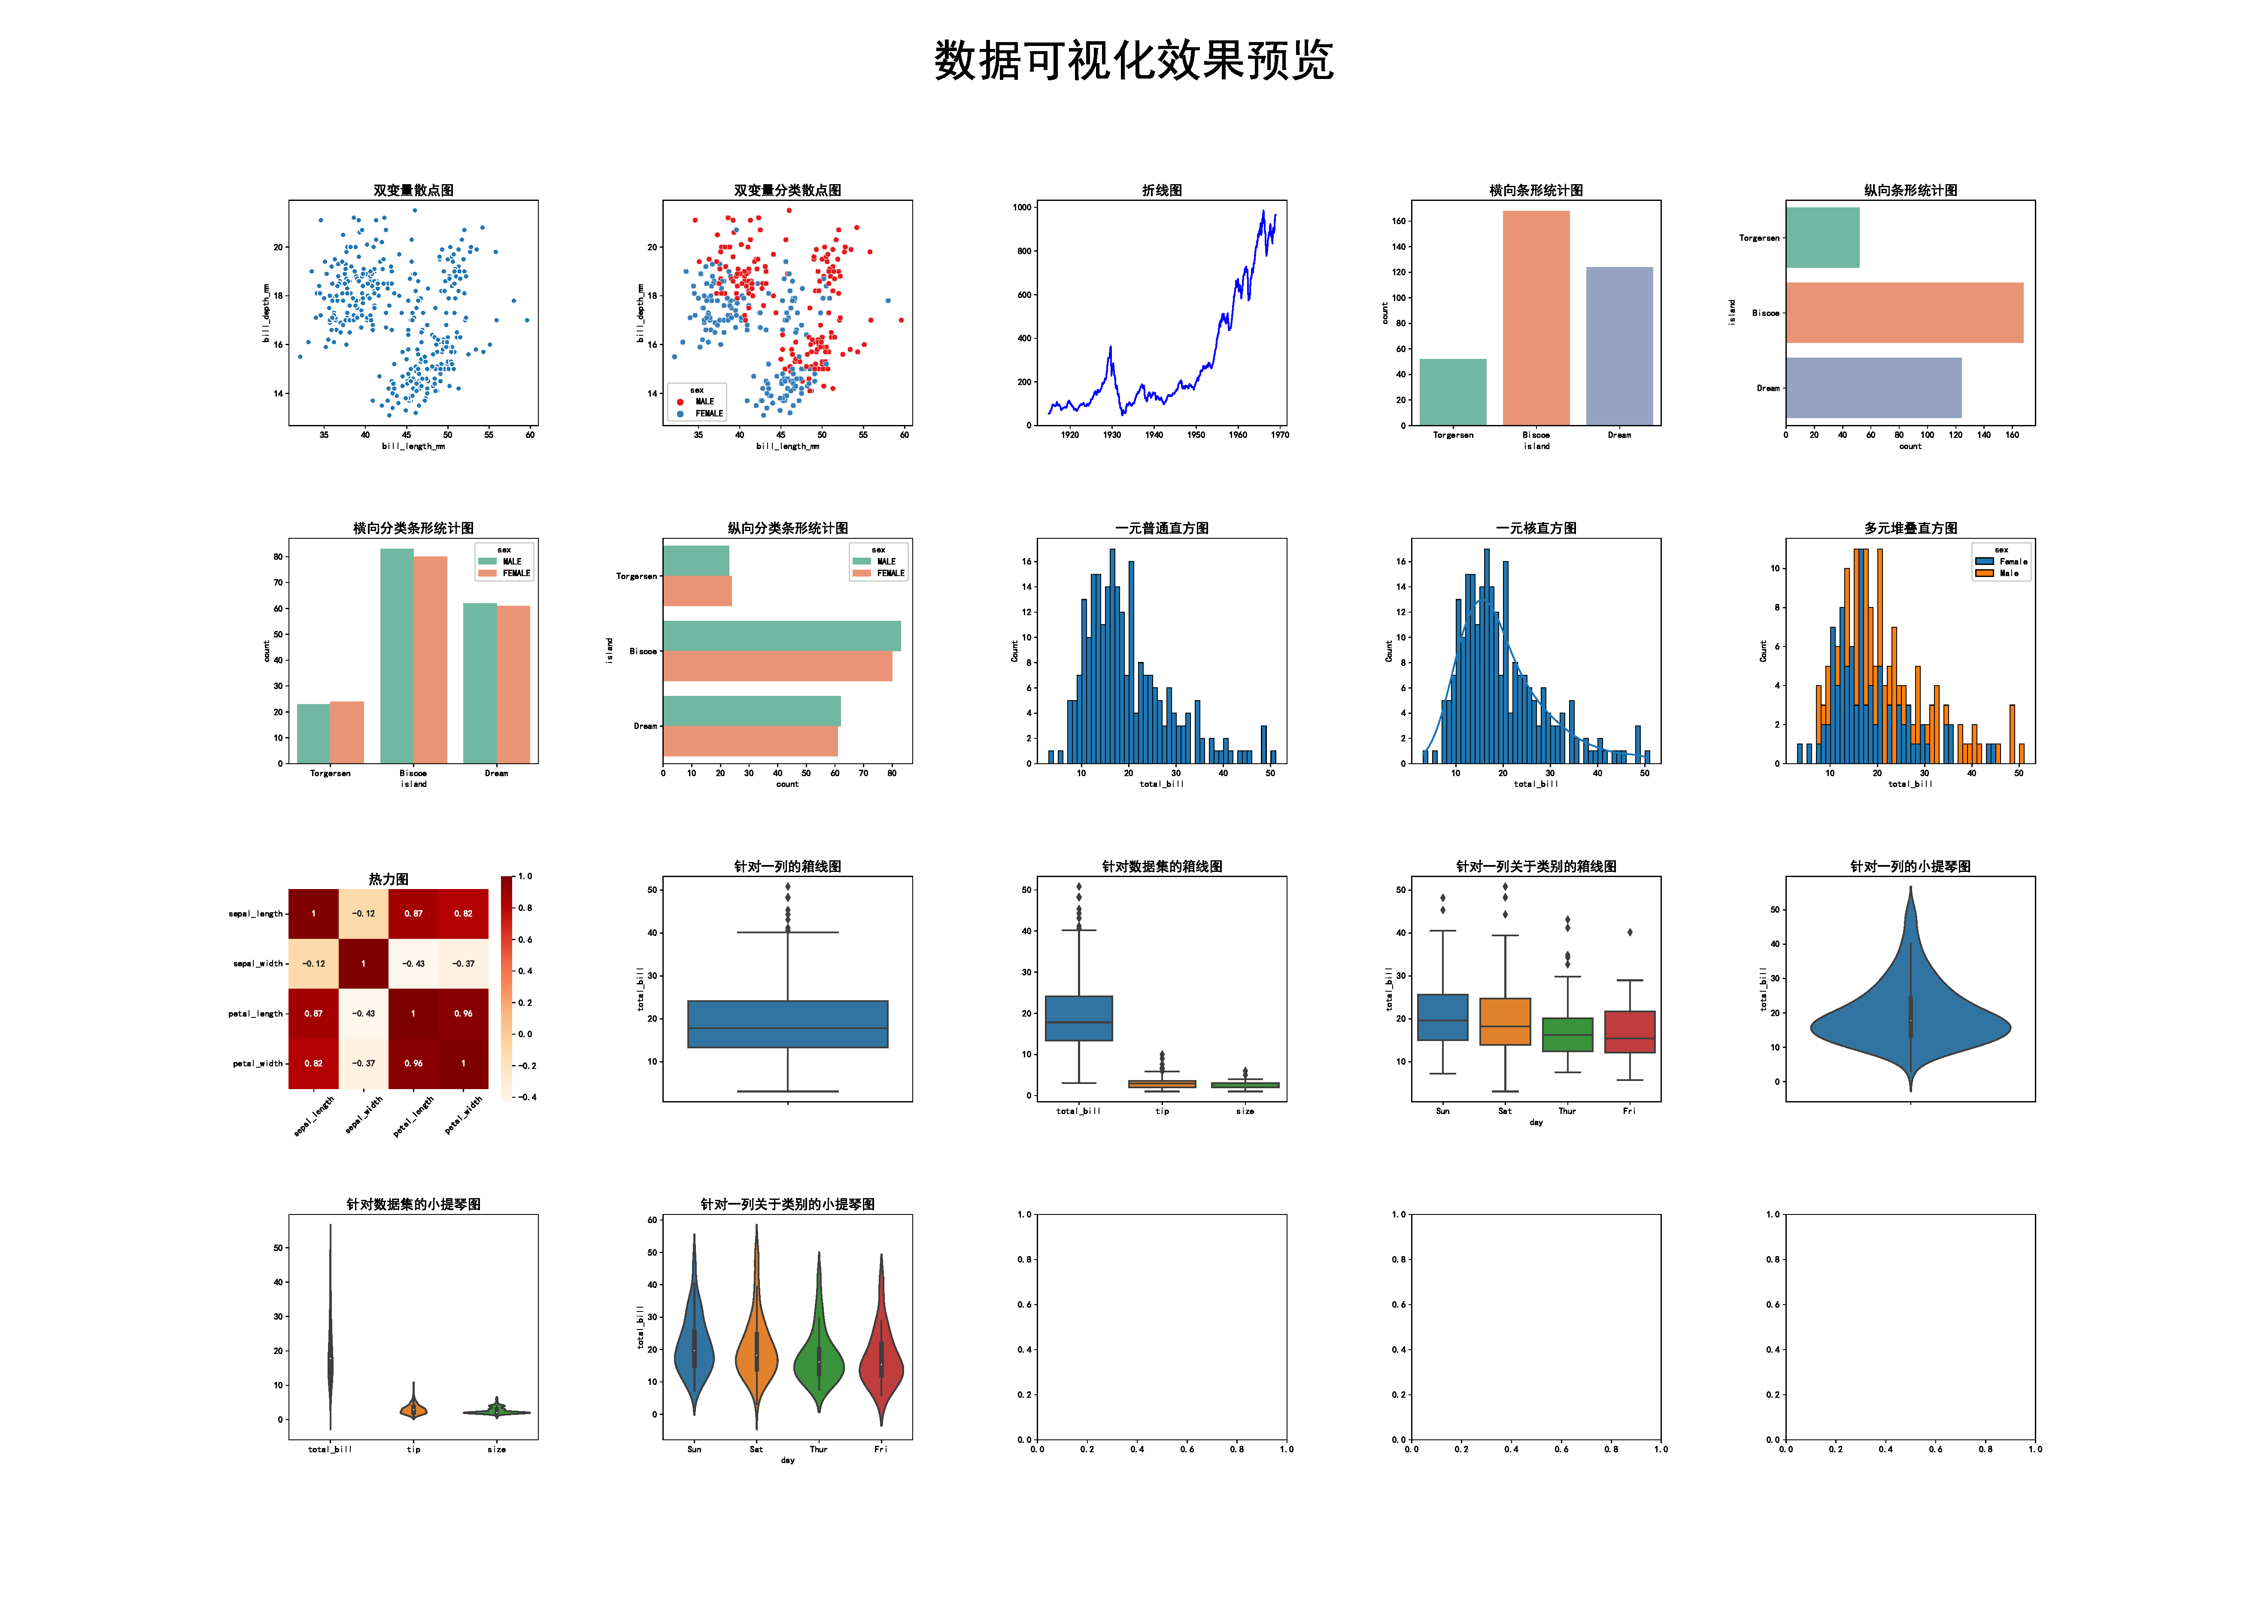
\includegraphics[width=1\textwidth]{1.eps}
	% 这是图注,也就是对图的解释,会在图片下方居中显示,请改成对应描述
	\caption{矢量图示例} 
	% 这是图片的标签,用于交叉引用该图片,务必全文唯一
	\label{fig2}
\end{figure}


矢量图也可以是pdf格式,比如本文的流程图——图~\ref{fig300}~就是pdf格式的。如果你希望在一行放多张图,可以参照图~\ref{fig100}~,~\ref{fig101}~:


\begin{figure}[H]
	\centering
	\begin{minipage}[t]{0.48\textwidth}
		\centering
		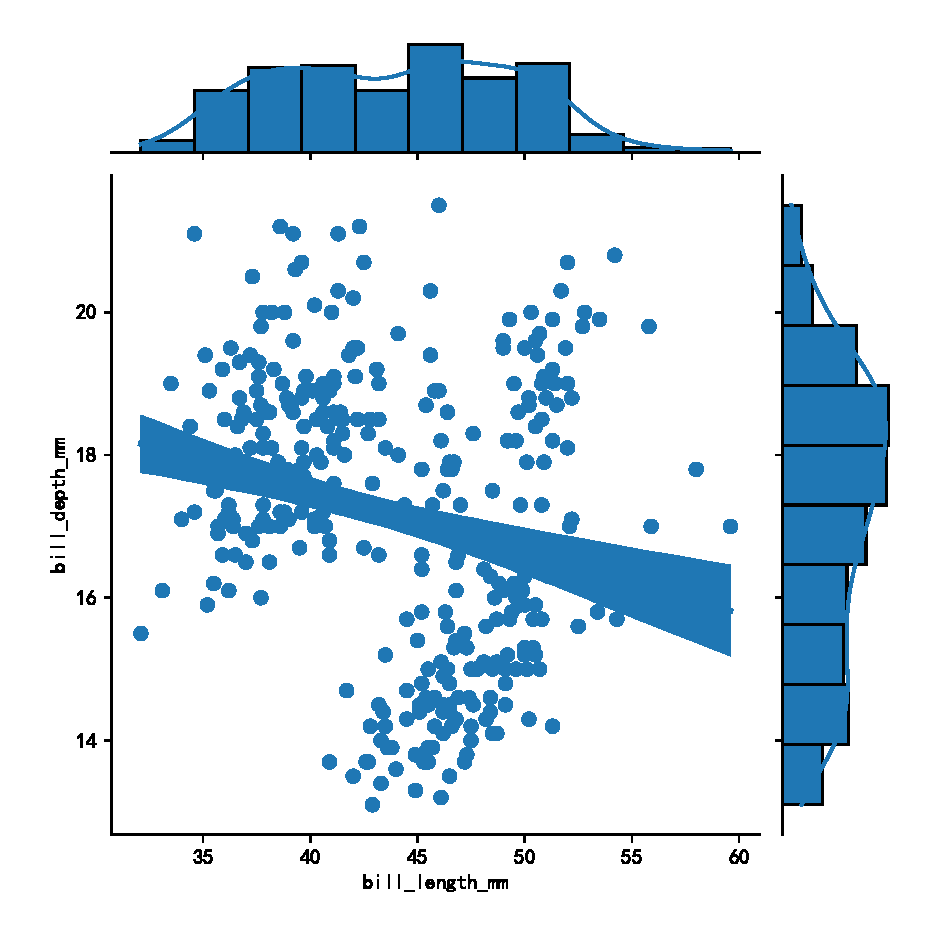
\includegraphics[width=1\textwidth]{test1.eps}
		\caption{左图}
		\label{fig100}
	\end{minipage}
	\begin{minipage}[t]{0.48\textwidth}
		\centering
		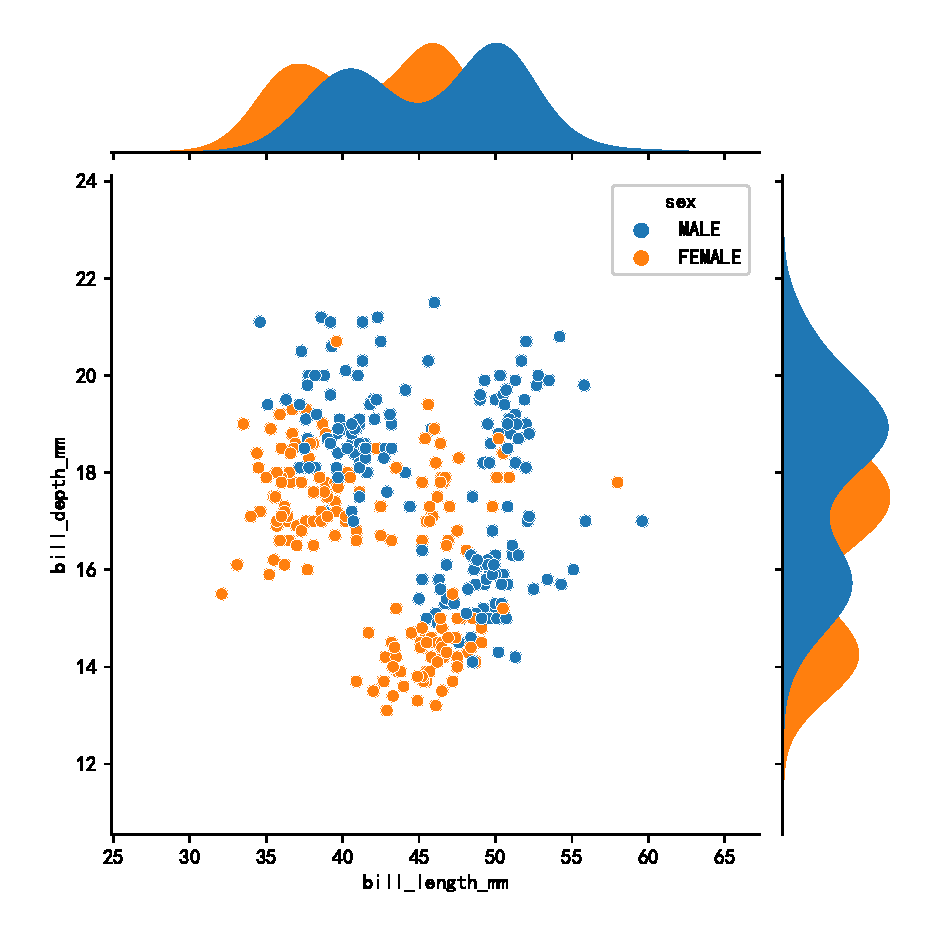
\includegraphics[width=1\textwidth]{test2.eps}
		\caption{右图}
		\label{fig101}
	\end{minipage}
\end{figure}

各位可以尝试一下,就会发现确有其事。

\subsection{插入表格}



论文中使用的表格一般是以三线表的形式呈现,三线表用处极多,必须掌握,而且在\LaTeX 中三线表是最麻烦的!我当初国赛通宵排版差点被三线表熬死,幸好孙竹清出手帮我搞定了,如表~\ref{table10}~:

\begin{table}[H]
	\centering
		\caption{这是表格标题。}
		\begin{tabular}{c c}  % 表有几列就要有几个c,c与c之间用空格隔开
			\toprule[1.5pt]   % 不要动
			% 表格内容,列与列之间用 & 隔开,一行内容写完了用 \\ 结束
			符号 & 含义  \\ 
			\midrule[1pt]     % 不要动
			$i=1,i=2$ & 分别表示高钾、铅钡玻璃 \\ 
			$j$ & 表示表中从二氧化硅($SiO_2$)到二氧化硫($SO_2$)中第$j$类化学物质 \\
			$z=1,z=2$ & 分别表示风化前和风化后 \\
			$x_1,x_2,x_3,x_4$ & 分别表示纹饰、类型、颜色、风化表面 \\
			$y_j$ & 表示第$j$类化学物质的含量 \\ 
			$\overline{y_j}$ & 表示第$j$类化学物质的平均含量 \\  
			\toprule[1.5pt]   % 不要动
		\end{tabular}
		\label{table10}
\end{table}

当然有时候也会遇到行合并单元格的情况,列合并的就比较少了,下面给出具体例子如表~\ref{table3}~:

\begin{table}[H]
	\centering
	\caption{对照组与实验组前、后测时间Mann-Whitney U检验}
	\begin{threeparttable}
		\begin{tabular}{c c c c c c c c c}
			\toprule[1.5pt]
			& 前测 & 平均值 & 标准差  & p值 & 后测 & 平均值 & 标准差  & p值 \\
			\midrule[1pt]
			
			
			\multirow{2}{*}{加法} & 对照组 & 某数据 & 某数据 & \multirow{2}{*}{某数据} & 对照组 & 某数据 & 某数据 & \multirow{2}{*}{某数据} \\
			
			& 实验组 & 某数据 & 某数据 &  & 实验组 & 某数据 & 某数据     \\
			
			\multirow{2}{*}{减法} & 对照组 & 某数据 & 某数据  & \multirow{2}{*}{某数据} & 对照组 & 某数据 & 某数据  & \multirow{2}{*}{某数据} \\
			
			& 实验组 & 某数据 & 某数据 &    & 实验组 & 某数据 & 某数据     \\
			\toprule[1.5pt]
		\end{tabular}
		\label{table3}
	\end{threeparttable}
\end{table}

我们在写论文时很可能会遇到极大量的计算结果需要放在三线表里,这个时候就很费心了,怎么办呢?在LaTeX中,你可以使用sidewaystable环境来创建一个横向表格,并且当表格横向放置不够时,自动将其旋转为竖向放置。你需要导入rotating宏包来使用这个环境。如表~\ref{table2}~所示:

\begin{table}[H]
	\centering
	\caption{这是一个横向的大表格}
	\begin{sideways}
		\begin{tabular}{c c c c c c c c c c c c c}
			\toprule[1.5pt]  
			列1 & 列2 & 列3 & 列1 & 列2 & 列3 列1 & 列2 & 列3 列1 & 列2 & 列3 列1 & 列2 & 列3 & 列1  \\
			\midrule[1pt]  
			内容1 & 内容2 & 内容3 & 内容1 & 内容2 & 内容3 & 内容1 & 内容2 & 内容3 &内容1 & 内容2 & 内容3 & 内容1  \\
			
			内容1 & 内容2 & 内容3 & 内容1 & 内容2 & 内容3 & 内容1 & 内容2 & 内容3 &内容1 & 内容2 & 内容3 & 内容1  \\
			
			内容1 & 内容2 & 内容3 & 内容1 & 内容2 & 内容3 & 内容1 & 内容2 & 内容3 &内容1 & 内容2 & 内容3 & 内容1 \\
			
			内容1 & 内容2 & 内容3 & 内容1 & 内容2 & 内容3 & 内容1 & 内容2 & 内容3 &内容1 & 内容2 & 内容3 & 内容1 \\
			
			内容1 & 内容2 & 内容3 & 内容1 & 内容2 & 内容3 & 内容1 & 内容2 & 内容3 &内容1 & 内容2 & 内容3 & 内容1  \\
			
			内容1 & 内容2 & 内容3 & 内容1 & 内容2 & 内容3 & 内容1 & 内容2 & 内容3 &内容1 & 内容2 & 内容3 & 内容1  \\
			
			内容1 & 内容2 & 内容3 & 内容1 & 内容2 & 内容3 & 内容1 & 内容2 & 内容3 &内容1 & 内容2 & 内容3 & 内容1  \\
			
			内容1 & 内容2 & 内容3 & 内容1 & 内容2 & 内容3 & 内容1 & 内容2 & 内容3 &内容1 & 内容2 & 内容3 & 内容1  \\
			
			内容1 & 内容2 & 内容3 & 内容1 & 内容2 & 内容3 & 内容1 & 内容2 & 内容3 &内容1 & 内容2 & 内容3 & 内容1  \\
			
			内容1 & 内容2 & 内容3 & 内容1 & 内容2 & 内容3 & 内容1 & 内容2 & 内容3 &内容1 & 内容2 & 内容3 & 内容1  \\
			
			内容1 & 内容2 & 内容3 & 内容1 & 内容2 & 内容3 & 内容1 & 内容2 & 内容3 &内容1 & 内容2 & 内容3 & 内容1  \\
			\toprule[1.5pt] 
			% 继续添加更多行和列
		\end{tabular}
	\end{sideways}
	\label{table2}
\end{table}



% ------------------------------------------------------------ %
%    打开chapter文件夹里的“7-问题三建模.tex”文件,编辑其中的内容
% ------------------------------------------------------------ %
\section{问题三的建模与求解(23华中赛B题问题3示例)}



\subsection{数据预处理}

\subsubsection{数据清洗与特征编码}

本问要求对根据用药信息和患者信息对给药后 3 分钟以内的 IPI 数据进行预测,通过观察附件2发现只需要提取出IPI005、IPI1、IPI015、IPI2、IPI025、IPI3的相关数据,并从原始数据集中筛选出了需要的特征作为特征空间——包括性别、年龄、身高、体重、有无手术史、是否吸烟、是否酗酒、镇静药名称、镇静药诱导剂量、有无追加镇静、镇静药总剂量、镇痛药总剂量。

与上文数据预处理类似地,基于Pandas查找缺失值并删除一些对模型预测没有意义的特征,包括手术说明、既往史说明、ASA评分等,之后删除少量含有缺失值的行。对特征空间中的数值特征进行特征缩放中的数据归一化,以消除其量纲;对分类特征进行编码以转化为离散特征——这些特征包括性别、有无手术史等。

\subsubsection{数据降维}

由于数据集中有大量的分类特征导致数据集整体较为离散,模型难以充分提取特征,且容易过拟合。使用主成分分析法对处理后数据进行降维,当前数据共有14列,通过将方差解释比例可视化可得下图:

\begin{figure}[H] % 这个H不要动!
	\centering % 不要动!
	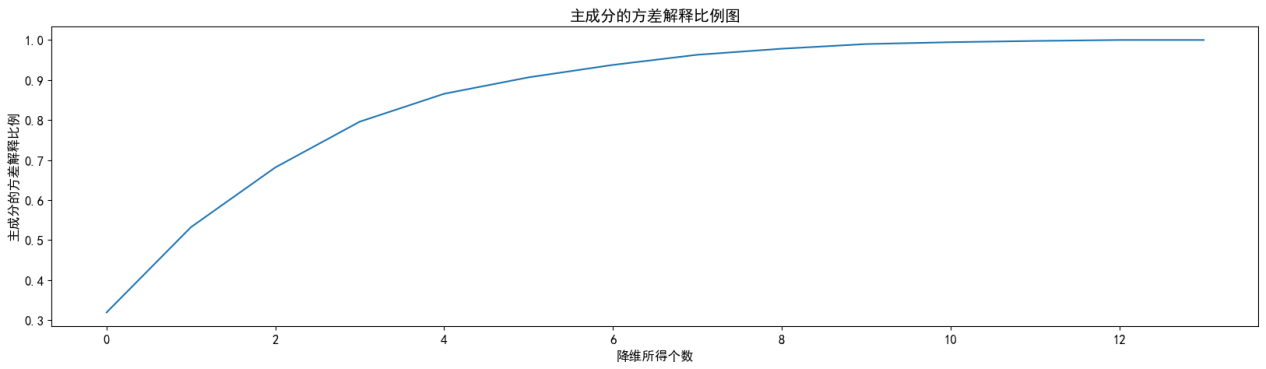
\includegraphics[width=0.95\textwidth]{8.png} 
	\caption{累积方差解释比例图} 
	\label{Fig.main8} 
\end{figure}

通过上图发现前四个主成分即可表示样本80\%的信息,因此保留了4个主成分,对4个主成分特征重新导入到数据集,便于后面利用监督学习中的回顾方法。

\subsection{岭回归与支持向量机回归的加权平均预测}


\subsubsection{模型建立}

\textbf{(一)岭回归模型}

\begin{enumerate}
	\item \textbf{岭回归}
	
	设有一个线性回归模型:
	
	\begin{equation}
		y=\overrightarrow{X}\overrightarrow{\beta }+\overrightarrow{\varepsilon }.
	\end{equation}
	其中,$\overrightarrow{X}$是$n\times p$的自变量矩阵,$\overrightarrow{\beta }$是$p$维系数向量,$y$是$n$维因变量向量,$\overrightarrow{\varepsilon }$是$n$维误差向量。
	
	引入L2正则化项后,岭回归的目标函数为:
	
	\begin{equation}
		\underset{\overrightarrow{\beta }}{\mathop{\min }}\,\left\{ \sum\limits_{i=1}^{n}{{{\left( {{y}_{i}}-\overrightarrow{x}_{i}^{T}\overrightarrow{\beta } \right)}^{2}}+\lambda \sum\limits_{j=1}^{p}{\overrightarrow{\beta }_{j}^{2}}} \right\}.
	\end{equation}
	其中,$\lambda$是正则化强度超参数,控制正则化项的权重大小。岭回归的解可以用闭式解表达式表示:
	
	\begin{equation}
		\widehat{\overrightarrow{\beta }}={{\left( {{\overrightarrow{X}}^{T}}\overrightarrow{X}+\lambda \overrightarrow{I} \right)}^{-1}}{{\overrightarrow{X}}^{T}}y.
	\end{equation}
	
	其中,$\overrightarrow{I}$是$p\times p$的单位矩阵。当$\lambda =0$时,岭回归就退化成了普通的线性回归;当$\lambda$取值较大时,正则化项的影响就越大,模型的系数就越接近于0。
	
	
	
	\item \textbf{支持向量机模型}
	
	对于数据集$D=\left\{ \left( {{\overrightarrow{x}}_{1}},{{y}_{1}} \right),\left( {{\overrightarrow{x}}_{2}},{{y}_{2}} \right),\cdots ,\left( {{\overrightarrow{x}}_{m}},{{y}_{m}} \right) \right\},$ ,得到一个回归模型$f\left( \overrightarrow{x} \right)$与$y$尽可能接近.SVR问题可形式化为:
	
	\begin{equation}
		f\left( \overrightarrow{x} \right)={{\overrightarrow{\omega }}^{T}}\Phi \left( \overrightarrow{x} \right)+b.
	\end{equation}
	
	\begin{equation}
		\overrightarrow{\omega }=\sum\limits_{i=1}^{m}{\left( {{\widehat{\alpha }}_{i}}-{{\alpha }_{i}} \right)\Phi \left( {{\overrightarrow{x}}_{i}} \right)}.
	\end{equation}
	
	\begin{equation}
		f\left( \overrightarrow{x} \right)=\sum\limits_{i=1}^{m}{\left( {{\widehat{\alpha }}_{i}}-{{\alpha }_{i}} \right)\kappa \left( \overrightarrow{x},{{\overrightarrow{x}}_{i}} \right)}+b.
	\end{equation}
	其中$\kappa \left( {{\overrightarrow{x}}_{i}},{{\overrightarrow{x}}_{j}} \right)=\Phi {{\left( {{\overrightarrow{x}}_{i}} \right)}^{T}}\Phi \left( {{\overrightarrow{x}}_{j}} \right)$为核函数.$\overrightarrow{\omega },b$为模型参数,${{\widehat{\alpha }}_{i}}\ge 0,{{\alpha }_{i}}\ge 0$是拉格朗日乘子.利用高斯核函数求解,公式为:
	
	\begin{equation}
		\kappa \left( {{\overrightarrow{x}}_{i}},{{\overrightarrow{x}}_{j}} \right)=\exp \left( -\frac{\left\| {{\overrightarrow{x}}_{i}}-{{\overrightarrow{x}}_{j}} \right\|}{2{{\sigma }^{2}}} \right).
	\end{equation}
	
\end{enumerate}





\subsubsection{模型求解}

首先基于Scikit-Learn建立三分钟内各时间点的IPI数值的两种预测模型——岭回归模型和SVR模型,设定岭回归模型在$i$样本的预测值为${{h}_{1}}({{\overrightarrow{x}}_{i}})$,SVR模型的预测值为${{h}_{2}}({{\overrightarrow{x}}_{i}}),i=1,2,\cdots ,m$,构建集成学习器$H$包含两个基学习器{${{h}_{1}},{{h}_{2}}$}。


对于题目中由已知的数据集进行建模,分别需要对六个标签——IPI005、IPI1、IPI015、IPI2、IPI025以及IPI3进行回归分析。加权平均法是一种常见的回归任务的模型融合方法,利用加权平均法进行结合,其中原理如下:

\begin{equation}
	{{\omega }_{i}}=\frac{MS{{E}_{i}}}{MS{{E}_{1}}+MS{{E}_{2}}},i=1,2.
\end{equation}


\begin{equation}
	H(\overrightarrow{x})=\frac{1}{2}\sum\limits_{i=1}^{2}{{{\omega }_{i}}{{h}_{i}}(\overrightarrow{x})}.
\end{equation}
其中,${{\omega }_{1}},{{\omega }_{2}}$分别表示两个模型的权重,通过计算两种模型集成后组成的最优模型$H(\overrightarrow{x})$。

对于两个基学习器和基于加权平均法的融合模型,本文分别在测试集上进行测试,基于MAE和MSE对模型泛化能力进行评价,所得如下:

\begin{table}[H]
	\centering  
	\caption{三种模型在测试集上的测试评价}
	\begin{tabular}{c c c c}  
		\toprule[1.5pt]  
		标签名称 & 模型 & MAE & MSE  \\  
		\midrule[1pt]    
		\multirow{3}{*}{IPI005} & 岭回归   & 0.1447	& 0.0423    \\ 
		& SVR      & 0.1418	& 0.0417    \\
		& 模型融合 & 0.1432	& 0.0419    \\
		\multirow{3}{*}{IPI1}   & 岭回归   & 0.2376	& 0.1020    \\ 
		& SVR      & 0.2272	& 0.1153    \\
		& 模型融合 & 0.2322	& 0.1066    \\
		\multirow{3}{*}{IPI015} & 岭回归   & 0.3669	& 0.1630	\\ 
		& SVR      & 0.3567	& 0.1808	\\
		& 模型融合 & 0.3570	& 0.1651	\\
		\multirow{3}{*}{IPI2}   & 岭回归   & 0.2666	& 0.1103	\\ 
		& SVR      & 0.2363	& 0.1174	\\
		& 模型融合 & 0.2509	& 0.1101	\\
		\multirow{3}{*}{IPI025} & 岭回归   & 0.1680	& 0.0679	\\ 
		& SVR      & 0.1663	& 0.0682	\\
		& 模型融合 & 0.1671	& 0.0678	\\
		\multirow{3}{*}{IPI3}   & 岭回归   & 0.1810	& 0.0798	\\ 
		& SVR      & 0.1788	& 0.0810	\\
		& 模型融合 & 0.1797	& 0.0800    \\
		\toprule[1.5pt]  
	\end{tabular}  
\end{table} 

分析上表可知,基于三种模型在测试集上的评价指标,对于这六种标签预测评价指标都接近0,说明这三种模型的预测效果都十分优良。从标签种类分析,可以发现对于标签IPI005的预测效果最佳,对于标签IPI015的预测效果最差。不同标签预测效果整体上的优良性从最优到优的排序为IPI005、IPI025、IPI3、IPI1、IPI2、IPI015。

分析三种模型发现无论是岭回归模型还是SVR模型都不能保证是性能最优,而将模型融合可以弥补单个模型的不足,提高准确率。同时提升模型的鲁棒性,降低由于数据的随机性导致的模型波动,得到的预测结果更准确,泛化能力更强,模型稳定性更强。模型融合是提高预测准确性、提高模型鲁棒性、降低模型波动性的一种有效方法。



\subsubsection{灵敏度分析}

为了评估两个不同的模型(Ridge回归和支持向量机)对输入数据的敏感性,这里通过施加一些高斯噪声(从0到0.5的比例),原理为

\begin{equation}
	f\left( x \right)=\frac{1}{\sigma \sqrt{2\pi }}{{e}^{-\frac{{{\left( x-\mu  \right)}^{2}}}{2{{\sigma }^{2}}}}}.
\end{equation}
其中,$x$表示随机变量的取值,$\mu$表示期望值,$\sigma$表示标准差。改变测试数据集的特征,来模拟模型的偏差,以确定模型的鲁棒性。然后根据分段函数:

\begin{equation}
	erro{{r}_{ij}}=\left\{ \begin{matrix}
		0  \\
		{{\overline{y}}_{ij}}+f({{x}_{j}})  \\
	\end{matrix} \right.\begin{matrix}
		,\left( 0,c \right)  \\
		,\left( c,0.5 \right)  \\
	\end{matrix}
\end{equation}
其中$\overline{y}_{ij}$为第$i$个特征的第$j$个的样本值,$f({{x}_{j}})$表示加入的高斯噪声,$c$表示噪音阈值。重新预测,并计算预测结果与真实结果之间的均方误差。下文以IPI3为例对模型灵敏度进行分析(其余见附件),得到数据可视化图如下所示:

\begin{figure}[H] % 这个H不要动!
	\centering % 不要动!
	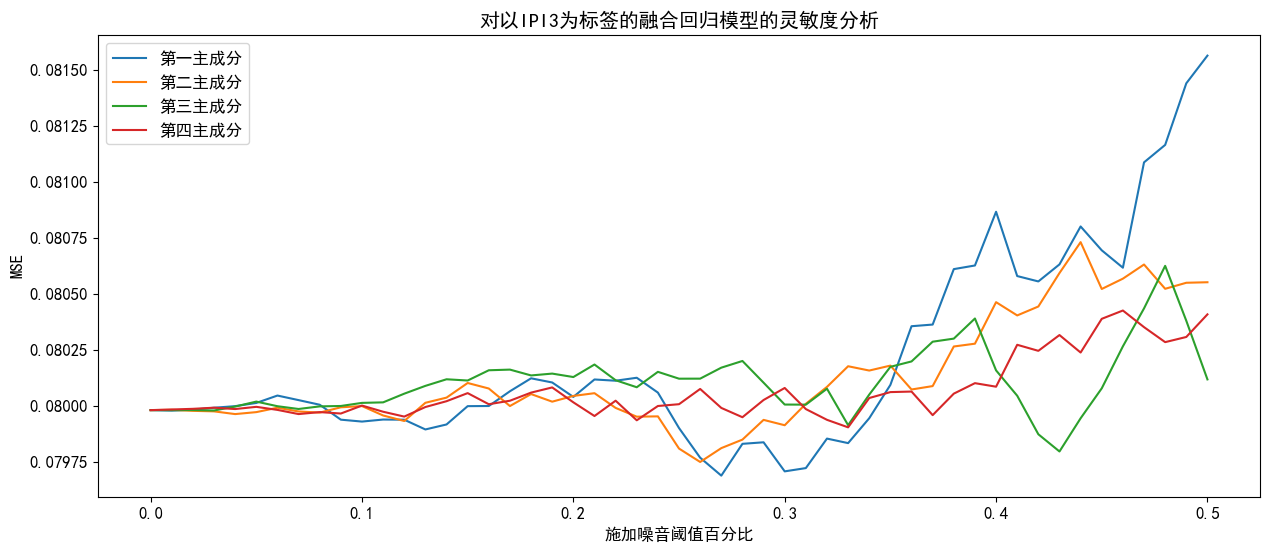
\includegraphics[width=0.95\textwidth]{9.png} 
	\caption{对以IPI3为标签的融合回归模型的灵敏度分析} 
	\label{Fig.main9} 
\end{figure}

从上图可以看出,对第一主成分、对第二主成分、对第三主成分、对第四主成分分别不断施加噪音,可以直观地看出MSE(均方差)值在这个区间波动,四个特征在施加噪音百分比在30\%以内时MSE均无明显波动,说明该模型具有一定的可靠性和稳定性性能优良。另外五个标签的灵敏度分析图详见附录A。



% ------------------------------------------------------------ %
%    打开chapter文件夹里的“8-模型评价.tex”文件,编辑其中的内容
% ------------------------------------------------------------ %
\section{模型评价和改进}

% 本章内容是要从宏观解释本文模型的厉害之处,本来是可以不写缺点的,一般写2个部分:优点、推广,下面我给的案例是我2022年国赛写的,初生牛犊不怕虎,写了缺点,本来当时是可以写基于Voting的推广的,但是国赛要求的篇幅,当时已经不够用了,所以作罢!


\subsection{模型优点}

\begin{enumerate}
	\item 在问题一中对文物表面是否风化与类型、颜色、纹饰关系分析过程中,不仅对于单变量之间进行了分析,还进一步用树模型进行了多变量与单变量的分析,同时利用互信息进一步对结果进行检验,提高模型的合理性。
	\item 本文做了大量图表来统计分析数据特点,直观的对比出两类玻璃风化前后的化学成分的变化量以及各类玻璃化学成分之间的关系。
	\item 在文本中多次对模型进行调参,利用混淆矩阵和多个指标检验,提高了模型的准确性。
	\item 使用强分类器,构建Voting集成算法,得到一个完美模型,得到结果可信度高。
\end{enumerate}



\subsection{模型缺点}

\begin{enumerate}
	\item 做编码时由于颜色样本有7个非叙述类别,而数据集中存在大量的分类特征,没有找到合理高效的特征编码方式。
\end{enumerate}


% \subsection{模型改进}

% \subsection{模型推广}


% ------------------------------------------------------------ %
%    打开chapter文件夹里的“9-参考文献.tex”文件,编辑其中的内容
% ------------------------------------------------------------ %
\section{参考文献}


% -------改下面的参考文献内容就行,别动这两句话!!!------- %
\renewcommand{\refname}{}
\vspace{-3em}  
% -------改下面的参考文献内容就行,别动这两句话!!!------- %


\begin{thebibliography}{200}  
	\bibitem{ref1}
	伏修锋,干福熹.基于多元统计分析方法对一批中国南方和西南地区的古玻璃成分的研究[J].文物保护与考古学2006(04).
	
	\bibitem{ref2}
	司守奎,孙玺菁.数学建模算法与应用(第3版)——北京:国防工业出版社,2021.4.
	
	\bibitem{ref3}
	周志华著;李楠译.集成学习:基础与算法——北京:电子工业出版社,2020.8. 
	
	\bibitem{ref4}
	司守奎,孙玺菁.Python数学建模算法与应用——北京:国防工业出版社,2022.1.
	
	\bibitem{ref5}
	王贺,刘鹏,钱乾著.机器学习算法竞赛实战——北京:人民邮电出版社,2021.9.
	
	\bibitem{ref6}
	何道江,黄旭东,张琼编.数学建模优秀论文选编——北京:科学出版社,2020.11.
	
	\bibitem{ref7}
	何伟,张良均主编.机器学习原理与实践——北京:人民邮电出版社,2021.7.
	
	\bibitem{ref8}
	孙玉林,余本国著.Python机器学习算法与实践——北京:电子工业出版社,2021,9.
\end{thebibliography} 


% ------------------------------------------------------------ %
%    打开chapter文件夹里的“10-附录.tex”文件,编辑其中的内容
% ------------------------------------------------------------ %
% -----------------------------------------------------
% 下面的附录格式仅供参考,说不定大家到时候时间太紧都
% 没时间写附录了,附录这部分是最开放的哈,想怎么写怎
% 么写,主要内容就是代码和你想放在文章里又没放的东西,
% 比如大型图表等。
% -----------------------------------------------------


% 别动!!!% 别动!!!
\appendix  % 别动!!!
% 别动!!!% 别动!!!




\section{附录:关键代码实现}

\subsection{描述性统计分析}


\begin{lstlisting}[language=Python]
print('Hello World!')
\end{lstlisting}



\subsection{数据可视化1}


\begin{lstlisting}[language=Python]
import pandas as pd
import numpy as np
import matplotlib.pyplot as plt
import seaborn as sns

plt.rcParams["font.sans-serif"] = ["SimHei"]
plt.rcParams['font.size'] = 12  # 字体大小
plt.rcParams['axes.unicode_minus'] = False  # 正常显示负号

XXXXXX

plt.figure(figsize=(8, 7))
plt.scatter(df['item_price'], df['ord_qty'], s=10, c='red')
plt.xlabel('item_price')
plt.ylabel('ord_qty')
plt.title("产品价格-需求量散点图")
plt.show()
\end{lstlisting}


\subsection{数据可视化2}


\begin{lstlisting}[language=Python]
import pandas as pd
import numpy as np
import matplotlib.pyplot as plt
import seaborn as sns

plt.rcParams["font.sans-serif"] = ["SimHei"]
plt.rcParams['font.size'] = 12  # 字体大小
plt.rcParams['axes.unicode_minus'] = False  # 正常显示负号

XXXXXX

plt.figure(figsize=(8, 7))
plt.scatter(df['item_price'], df['ord_qty'], s=10, c='red')
plt.xlabel('item_price')
plt.ylabel('ord_qty')
plt.title("产品价格-需求量散点图")
plt.show()
\end{lstlisting}



\subsection{数据可视化3}


\begin{lstlisting}[language=Python]
import pandas as pd
import numpy as np
import matplotlib.pyplot as plt
import seaborn as sns

plt.rcParams["font.sans-serif"] = ["SimHei"]
plt.rcParams['font.size'] = 12  # 字体大小
plt.rcParams['axes.unicode_minus'] = False  # 正常显示负号

XXXXXX

plt.figure(figsize=(8, 7))
plt.scatter(df['item_price'], df['ord_qty'], s=10, c='red')
plt.xlabel('item_price')
plt.ylabel('ord_qty')
plt.title("产品价格-需求量散点图")
plt.show()
\end{lstlisting}


\section{附录:图表(随便放的别当真)}

\begin{figure}[H] 
	\centering 
	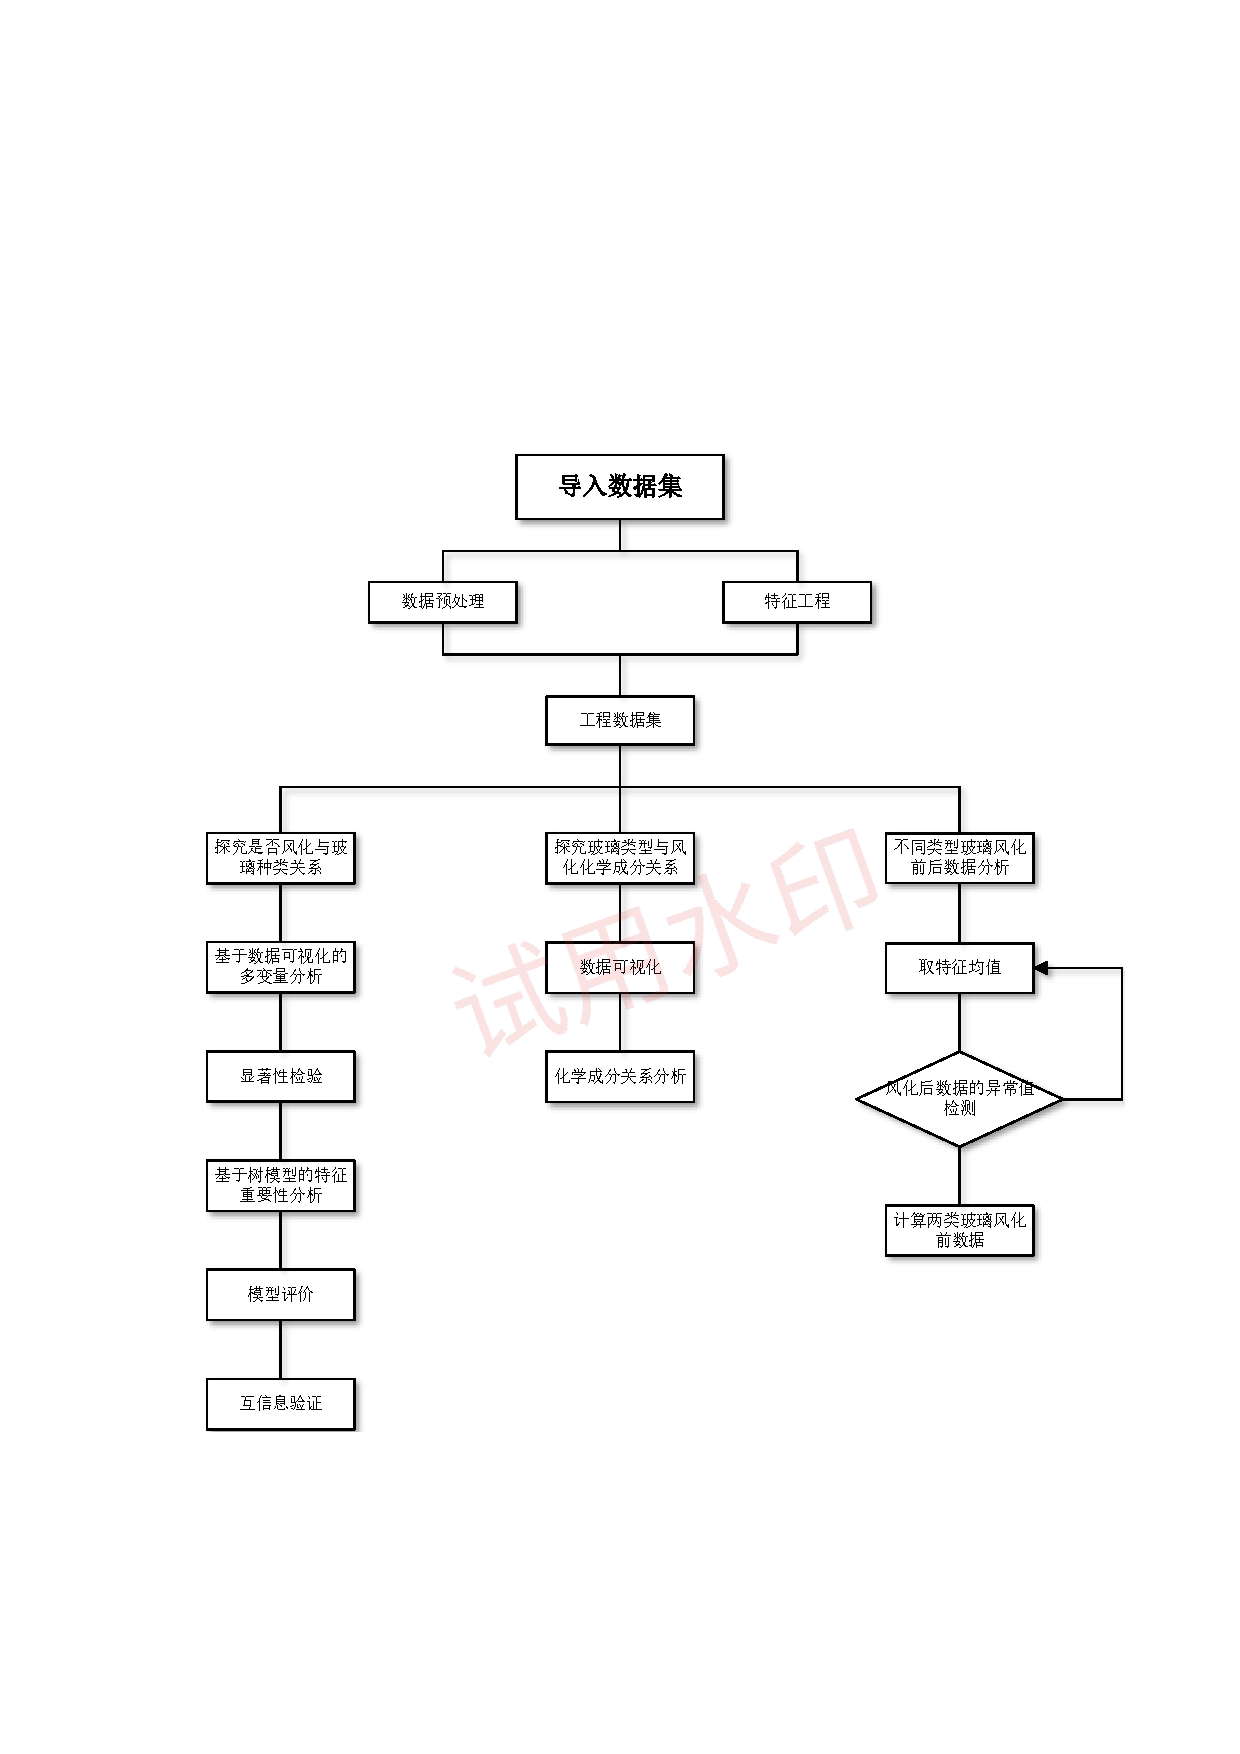
\includegraphics[width=0.95\textwidth]{1.pdf} 
	\caption{附录图表1} 
	\label{fig300} 
\end{figure}


\begin{table}[H]
	\centering
	\caption{附录图表1}
	\begin{tabular}{c c}
		\toprule[1.5pt]
		符号 & 含义  \\ 
		\midrule[1pt]
		$i=1,i=2$ & 分别表示高钾、铅钡玻璃 \\ 
		$j$ & 表示表中从二氧化硅($SiO_2$)到二氧化硫($SO_2$)中第$j$类化学物质 \\
		$z=1,z=2$ & 分别表示风化前和风化后 \\
		$x_1,x_2,x_3,x_4$ & 分别表示纹饰、类型、颜色、风化表面 \\
		$y_j$ & 表示第$j$类化学物质的含量 \\ 
		$\overline{y_j}$ & 表示第$j$类化学物质的平均含量 \\  
		\toprule[1.5pt]
	\end{tabular}
\end{table} 


\section{附录:图表(随便放的别当真)}

\begin{figure}[H] 
	\centering 
	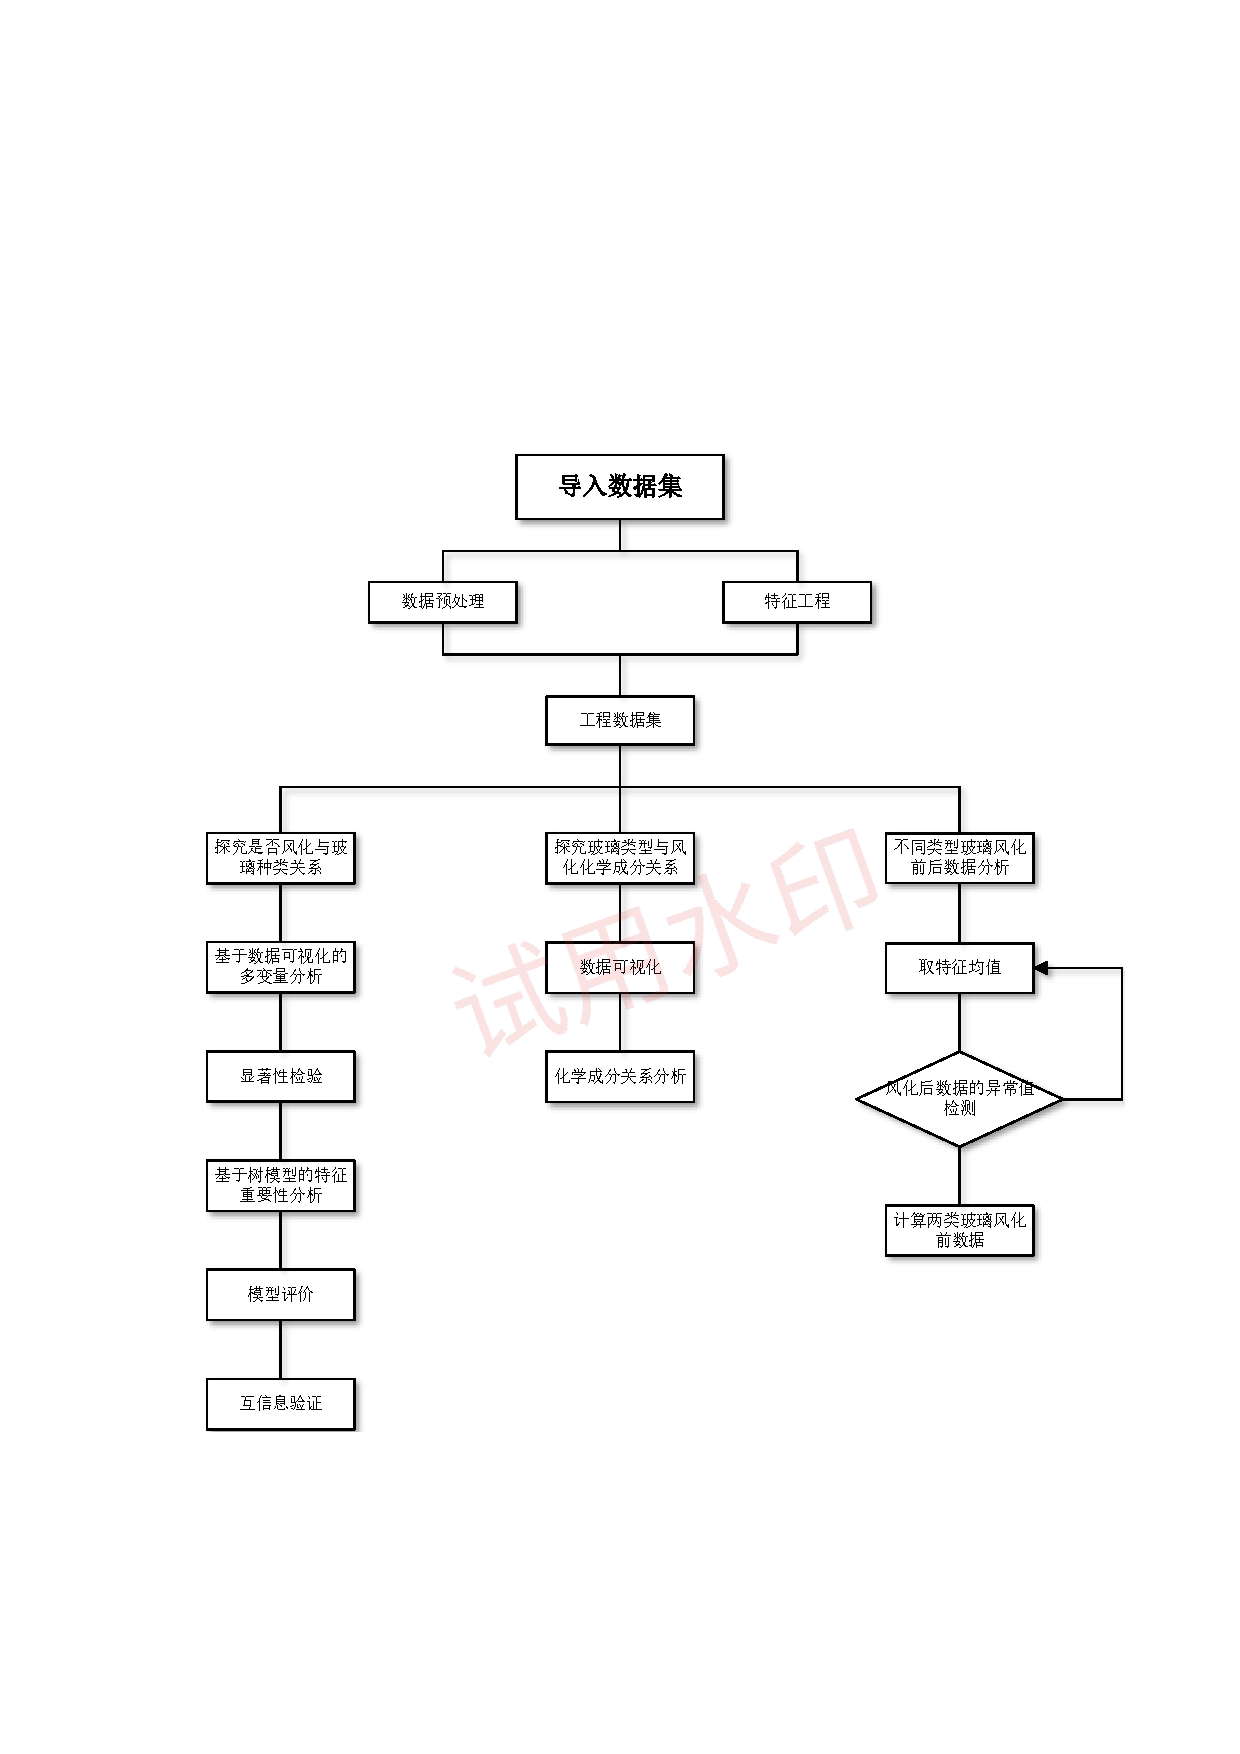
\includegraphics[width=0.95\textwidth]{1.pdf} 
	\caption{附录图表1} 
	\label{fig3000} 
\end{figure}


\begin{table}[H]
	\centering
	\caption{附录图表1}
	\begin{tabular}{c c}
		\toprule[1.5pt]
		符号 & 含义  \\ 
		\midrule[1pt]
		$i=1,i=2$ & 分别表示高钾、铅钡玻璃 \\ 
		$j$ & 表示表中从二氧化硅($SiO_2$)到二氧化硫($SO_2$)中第$j$类化学物质 \\
		$z=1,z=2$ & 分别表示风化前和风化后 \\
		$x_1,x_2,x_3,x_4$ & 分别表示纹饰、类型、颜色、风化表面 \\
		$y_j$ & 表示第$j$类化学物质的含量 \\ 
		$\overline{y_j}$ & 表示第$j$类化学物质的平均含量 \\  
		\toprule[1.5pt]
	\end{tabular}
\end{table} 


\end{document} 